% SC2002 --- Chapter 6: Design Patterns (Strategy/Observer/Factory)
\chapter{Design Patterns: Reusable Solutions (Strategy, Observer, Factory)}
\label{ch:patterns}

\begin{quote}
\emph{``A pattern is a solution to a problem in a context.''} --- Patterns name recurring design situations and their proven shapes. We study three workhorses---Strategy, Observer, and Factory---deeply enough to apply them, not just recite them.
\end{quote}

\noindent\fbox{\parbox{\dimexpr\linewidth-2\fboxsep-2\fboxrule}{%
\textbf{From zero: built on Ch.~1--5.} Each pattern is introduced as a concrete pain (switch, polling, scattered \texttt{new}) then solved. Only three patterns, fully worked with UML + Java + sequence traces.}}
\vspace{0.4em}

\section*{Learning Outcomes}
After this chapter you will be able to:
\begin{enumerate}[label=(L\arabic*)]
    \item state the intent, structure, and consequences of Strategy, Observer, and Factory (Method + Simple/Abstract);
    \item apply Strategy to eliminate switch-on-type and OCP violations;
    \item apply Observer for event-driven decoupling and explain push vs.\ pull and leak/lifecycle pitfalls;
    \item apply Factory to centralise creation, hide concrete types, and honour DIP;
    \item select among the three patterns (and recognise when \emph{no} pattern is needed).
\end{enumerate}

% ============================================================
\section{Strategy: Encapsulate What Varies}
\label{sec:strategy}
\emph{Problem:} behaviour varies by case and a \texttt{switch} grows with each new case (violates OCP). Example: shipping cost (Standard/Express/Overnight), discount rules, sorting comparators.

\emph{Solution:} define a \emph{Strategy} interface for the varying behaviour; each variant is a concrete strategy; the \emph{Context} holds a reference to the current strategy and delegates.

\begin{figure}[h]
\centering
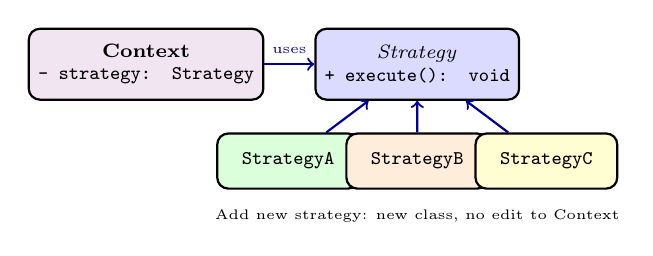
\begin{tikzpicture}[scale=0.82, every node/.style={font=\scriptsize}]
\node[draw,thick,fill=violet!10,rounded corners=4pt,minimum width=2.6cm,minimum height=0.9cm,align=center] (ctx) at (0,0) {\textbf{Context}\\\texttt{- strategy: Strategy}};
\node[draw,thick,fill=blue!14,rounded corners=4pt,minimum width=2.4cm,minimum height=0.9cm,align=center] (strat) at (4.2,0) {\textit{Strategy}\\\texttt{+ execute(): void}};
\node[draw,thick,fill=green!14,rounded corners=4pt,minimum width=1.8cm,minimum height=0.7cm] (a) at (2.2,-1.5) {\texttt{StrategyA}};
\node[draw,thick,fill=orange!14,rounded corners=4pt,minimum width=1.8cm,minimum height=0.7cm] (b) at (4.2,-1.5) {\texttt{StrategyB}};
\node[draw,thick,fill=yellow!18,rounded corners=4pt,minimum width=1.8cm,minimum height=0.7cm] (c) at (6.2,-1.5) {\texttt{StrategyC}};
\draw[->,thick,blue!60!black] (ctx) -- (strat) node[midway,above,font=\tiny] {uses};
\draw[->,thick,blue!60!black] (a) -- (strat);
\draw[->,thick,blue!60!black] (b) -- (strat);
\draw[->,thick,blue!60!black] (c) -- (strat);
\node[font=\tiny,fill=white,rounded corners=2pt,inner sep=2pt] at (4.2,-2.35) {Add new strategy: new class, no edit to Context};
\end{tikzpicture}
\caption{Strategy pattern: Context delegates to a Strategy interface; new behaviours are new classes (OCP).}
\label{fig:strategy-structure}
\end{figure}

\begin{lstlisting}[language=Java, caption={Strategy eliminates the switch and honours OCP.}]
interface ShippingStrategy { double cost(double weight); }
class StandardShipping implements ShippingStrategy { public double cost(double w){return 5+0.5*w;}}
class ExpressShipping  implements ShippingStrategy { public double cost(double w){return 12+1.2*w;}}
class Checkout {
    private ShippingStrategy shipping;
    public Checkout(ShippingStrategy s){ this.shipping=s; } // inject
    public void setShipping(ShippingStrategy s){ this.shipping=s; }
    public double total(double weight, double items){ return items + shipping.cost(weight); }
}
// Adding Overnight: new class, no edit to Checkout
class OvernightShipping implements ShippingStrategy { public double cost(double w){return 25+2.0*w;}}
\end{lstlisting}

% --- TikZ 2: Observer ---
\begin{figure}[h]
\centering
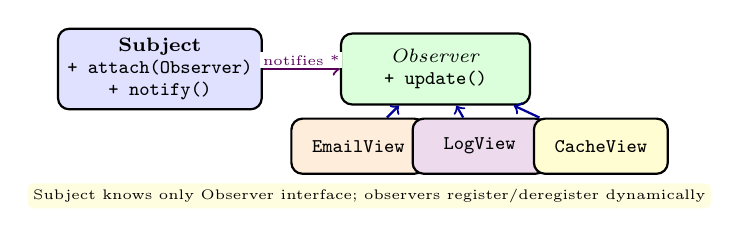
\begin{tikzpicture}[scale=0.70, every node/.style={font=\scriptsize}]
\node[draw,thick,fill=blue!12,rounded corners=4pt,minimum width=2.4cm,minimum height=0.9cm,align=center] (subj) at (0,0) {\textbf{Subject}\\\texttt{+ attach(Observer)}\\\texttt{+ notify()}};
\node[draw,thick,fill=green!14,rounded corners=4pt,minimum width=2.4cm,minimum height=0.9cm,align=center] (obs) at (5.0,0) {\textit{Observer}\\\texttt{+ update()}};
\node[draw,thick,fill=orange!14,rounded corners=4pt,minimum width=1.7cm,minimum height=0.7cm] (o1) at (3.6,-1.4) {\texttt{EmailView}};
\node[draw,thick,fill=violet!14,rounded corners=4pt,minimum width=1.7cm,minimum height=0.7cm] (o2) at (5.8,-1.4) {\texttt{LogView}};
\node[draw,thick,fill=yellow!18,rounded corners=4pt,minimum width=1.7cm,minimum height=0.7cm] (o3) at (8.0,-1.4) {\texttt{CacheView}};
\draw[->,thick,blue!60!black] (o1) -- (obs);
\draw[->,thick,blue!60!black] (o2) -- (obs);
\draw[->,thick,blue!60!black] (o3) -- (obs);
\draw[->,thick,violet!70!black] (subj) -- (obs) node[midway,above,font=\tiny,fill=white,inner sep=1pt] {notifies *};
\node[font=\tiny,fill=yellow!12,rounded corners=2pt,inner sep=2pt] at (3.8,-2.3) {Subject knows only Observer interface; observers register/deregister dynamically};
% sequence hint
\end{tikzpicture}
\caption{Observer: Subject maintains a list of Observers and notifies them on state change. Decouples event source from event consumers.}
\label{fig:observer-structure}
\end{figure}

\section{Observer: Decouple Event Source from Consumers}
\label{sec:observer}
\emph{Problem:} many views depend on one model's state (UI, cache, audit log). Polling is wasteful; direct calls couple model to every view.

\emph{Solution:} \emph{Subject} holds a list of \texttt{Observer}s; on change it calls \texttt{notify()} which invokes \texttt{update()} on each observer. Observers register/unregister at runtime.

\begin{lstlisting}[language=Java, caption={Observer with push vs.\ pull and lifecycle.}
]
interface Observer { void update(Book b); } // push: subject pushes data
class BookStore { // Subject
    private List<Observer> observers = new ArrayList<>();
    private List<Book> books = new ArrayList<>();
    public void attach(Observer o){ observers.add(o); }
    public void detach(Observer o){ observers.remove(o); }
    public void addBook(Book b){ books.add(b); notifyObservers(b); }
    private void notifyObservers(Book b){ for(Observer o: observers) o.update(b); }
}
class AvailabilityView implements Observer {
    public void update(Book b){ System.out.println(b.getTitle()+" now available"); }
}
\end{lstlisting}

Pitfalls: forgetting to \texttt{detach} leaks observers (memory leak, stale updates); notifying while holding a lock can deadlock; ordering of notification may matter. Java provides \texttt{PropertyChangeListener} / reactive streams for production use.

% --- TikZ 3: Factory ---
\begin{figure}[h]
\centering
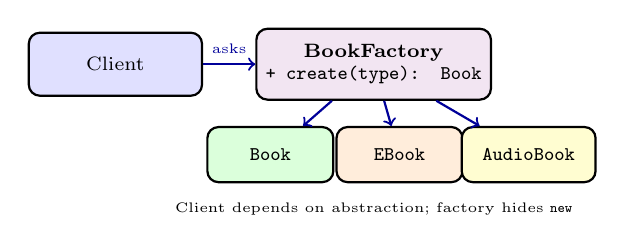
\begin{tikzpicture}[scale=0.82, every node/.style={font=\scriptsize}]
\node[draw,thick,fill=blue!12,rounded corners=4pt,minimum width=2.2cm,minimum height=0.8cm] (client) at (0,0) {Client};
\node[draw,thick,fill=violet!10,rounded corners=4pt,minimum width=2.4cm,minimum height=0.9cm,align=center] (factory) at (4.0,0) {\textbf{BookFactory}\\\texttt{+ create(type): Book}};
\node[draw,thick,fill=green!14,rounded corners=4pt,minimum width=1.6cm,minimum height=0.7cm] (b) at (2.4,-1.4) {\texttt{Book}};
\node[draw,thick,fill=orange!14,rounded corners=4pt,minimum width=1.6cm,minimum height=0.7cm] (e) at (4.4,-1.4) {\texttt{EBook}};
\node[draw,thick,fill=yellow!18,rounded corners=4pt,minimum width=1.7cm,minimum height=0.7cm] (a) at (6.4,-1.4) {\texttt{AudioBook}};
\draw[->,thick,blue!60!black] (client) -- (factory) node[midway,above,font=\tiny] {asks};
\draw[->,thick,blue!60!black] (factory) -- (b);
\draw[->,thick,blue!60!black] (factory) -- (e);
\draw[->,thick,blue!60!black] (factory) -- (a);
\node[font=\tiny,fill=white,rounded corners=2pt,inner sep=2pt] at (4.0,-2.25) {Client depends on abstraction; factory hides \texttt{new}};
\end{tikzpicture}
\caption{Factory: centralise creation so clients depend on abstractions, not concrete constructors. Abstract Factory generalises to families.}
\label{fig:factory-structure}
\end{figure}

\section{Factory: Centralise Creation}
\label{sec:factory}
\emph{Problem:} \texttt{new} scattered across the codebase couples clients to concrete classes and duplicates creation logic (validation, caching, subtypes).

\emph{Solution:} a \emph{Factory} encapsulates creation: \texttt{Simple Factory} (one method with a type flag), \emph{Factory Method} (subclasses decide which product to create), \emph{Abstract Factory} (families of related products).

\begin{lstlisting}[language=Java, caption={Simple Factory and Factory Method.}]
// Simple Factory: one place to change when construction changes
class BookFactory {
    public static Book create(String type, String title){
        return switch(type){
            case "ebook" -> new EBook(title, "https://...");
            case "audio" -> new AudioBook(title, 3600);
            default      -> new Book(title);
        };
    }
}
// Factory Method: subclasses override creation
abstract class LibraryImporter {
    public void importAll(){ Book b = createBook(); /* common logic */ }
    protected abstract Book createBook();
}
class EBookImporter extends LibraryImporter { protected Book createBook(){return new EBook("t","url");}}
\end{lstlisting}

Factories also enable DIP: high-level code asks the factory for a \texttt{Book}, never mentioning \texttt{EBook} directly; test code injects a factory that returns mocks.

\begin{remark}[When not to pattern]
If you have one shipping rule and no second one on the horizon, a simple \texttt{if} is clearer than Strategy. Patterns pay off at the second or third variant (Rule of Three). Do not apply patterns speculatively.
\end{remark}

\section{Choosing and Combining Patterns}
\label{sec:choosing-patterns}
\paragraph{Decision guide.}
\begin{itemize}[itemsep=0.25em]
    \item Varying \emph{algorithm/behaviour} chosen at runtime? $\to$ \textbf{Strategy} (or lambda).
    \item One-to-many event notification, runtime subscribers? $\to$ \textbf{Observer}.
    \item Creation is complex, varies by type/family, or must hide concrete classes? $\to$ \textbf{Factory}.
\end{itemize}

\paragraph{Combinations.} Patterns compose. A Factory often creates Strategies (\texttt{ShippingFactory.create("express")}); an Observer's Subject may be created by a Factory; Strategy objects can be Observers. Recognising composition is more valuable than memorising 23 names.

\begin{lstlisting}[language=Java, caption={Patterns compose: Factory creates the right Strategy at runtime.}]
class ShippingFactory {
    static ShippingStrategy of(String type){
        return switch(type){
            case "standard" -> new StandardShipping();
            case "express"  -> new ExpressShipping();
            case "overnight"-> new OvernightShipping();
            default -> throw new IllegalArgumentException("unknown: "+type);
        };
    }
}
class Checkout2 {
    double total(String shipType, double w, double items){
        return items + ShippingFactory.of(shipType).cost(w); // OCP + centralised creation
    }
}
\end{lstlisting}

\paragraph{Modern Java notes.} Since Java 8, Strategy is often a \texttt{Function} or method reference; Observer is often a \texttt{Flow.Publisher} or event bus; Factory benefits from \texttt{Supplier<T>} and dependency injection frameworks. The \emph{ideas} outlive the boilerplate.

\begin{remark}[Anti-patterns]
Over-applying patterns is a smell: ``FactoryFactory'' indirection, Observer chains that become callback hell, and Strategy proliferation where a simple \texttt{if} would suffice. Apply the simplest thing that honours the principles (Ch.~5).
\end{remark}

\section{Chapter Notes}
Gamma et al.\ \emph{Design Patterns} (1994) catalogued 23 patterns; we cover three with highest frequency in application code. Head First Design Patterns (Freeman \& Robson) has approachable elaborations. Modern Java often replaces Strategy with lambdas (\texttt{Function}) and Observer with \texttt{Flow}/reactive streams---same ideas, lighter syntax.

\section{Exercises}
\label{sec:ch06-exercises}
\begin{enumerate}[label=E6.\arabic*, leftmargin=*, itemsep=0.8em]
    \item \textbf{Strategy refactor.} Refactor a \texttt{calculateFee(MemberType type)} switch with cases \texttt{STUDENT, STAFF, PUBLIC} to Strategy. Show the interface, three strategies, and how \texttt{FeeCalculator} is now OCP-compliant.
    \item \textbf{Observer leak.} An Android Activity registers as observer in \texttt{onCreate} but never unregisters. Explain the leak, when it manifests, and fix with \texttt{detach} in the lifecycle. How would a weak-reference observer list help?
    \item \textbf{Push vs.\ pull.} Compare push (\texttt{update(Book b)}) vs.\ pull (\texttt{update()} then \texttt{subject.getState()}) for Observer. When does each win? Illustrate with a stock-ticker vs.\ large document model.
    \item \textbf{Factory vs.\ constructor.} A client does \texttt{new EBook(...)} in five places. A new requirement adds authentication tokens to every EBook. Show how Simple Factory reduces the change to one place and how it improves testability with a mock factory.
    \item \textbf{Pattern selection.} For each requirement say which pattern (if any) fits and why: (a) support PayNow, PayLah!, and credit-card payments; (b) notify three UIs when a loan becomes overdue; (c) create families of UI widgets per OS theme (light/dark). Justify with intent matching.
\end{enumerate}
% End of Chapter 6
